\chapter{Atome und Moleküle}

\section{Der Photoeffekt}
Bestrahlt man die Oberfläche eines Metalles mit Photonen, so werden Elektronen aus dieser herausgelöst.
Im Rahmen der klassischen Physik erscheinen bei diesem Versuch folgende Resultate als verwunderlich:
\begin{itemize}
	\item Die kinetische Energie der herausgelösten Elektronen hängt nicht von der Bestrahlungsstärke des Lichtes ab, sondern alleine von dessen Wellenlänge.
	\item Die kinetische Energie der Photoelektronen steigt ab einer Grenzfrequenz linear mit der Frequenz des Lichtes an.
	\item Die Grenzfrequenz hängt dabei nur vom Material der Kathodenoberfläche ab (Austrittsarbeit)
	\item Die Freisetzung der Elektronen beginnt instantan mit dem Einfall des Lichtes und endet genauso schnell auch mit dem Ende der Bestrahlung.
\end{itemize}

Man führt diese Beobachtungen auf den Teilchencharakter des Lichtes zurück.
Die Quantenmechanik konnte dabei erst den Welle-Teilchen-Dualismus des Lichtes deuten.

\section{Der Franck-Hertz-Versuch}
\begin{figure}
	\centering
	\begin{subfigure}{0.4\textwidth}
		\centering
		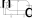
\includegraphics[width=\textwidth]{./img/fhversuch.pdf}
		\caption{Der Versuchsaufbau}
		\label{fig:fhversuch}
	\end{subfigure}
	\begin{subfigure}{0.4\textwidth}
		\centering
		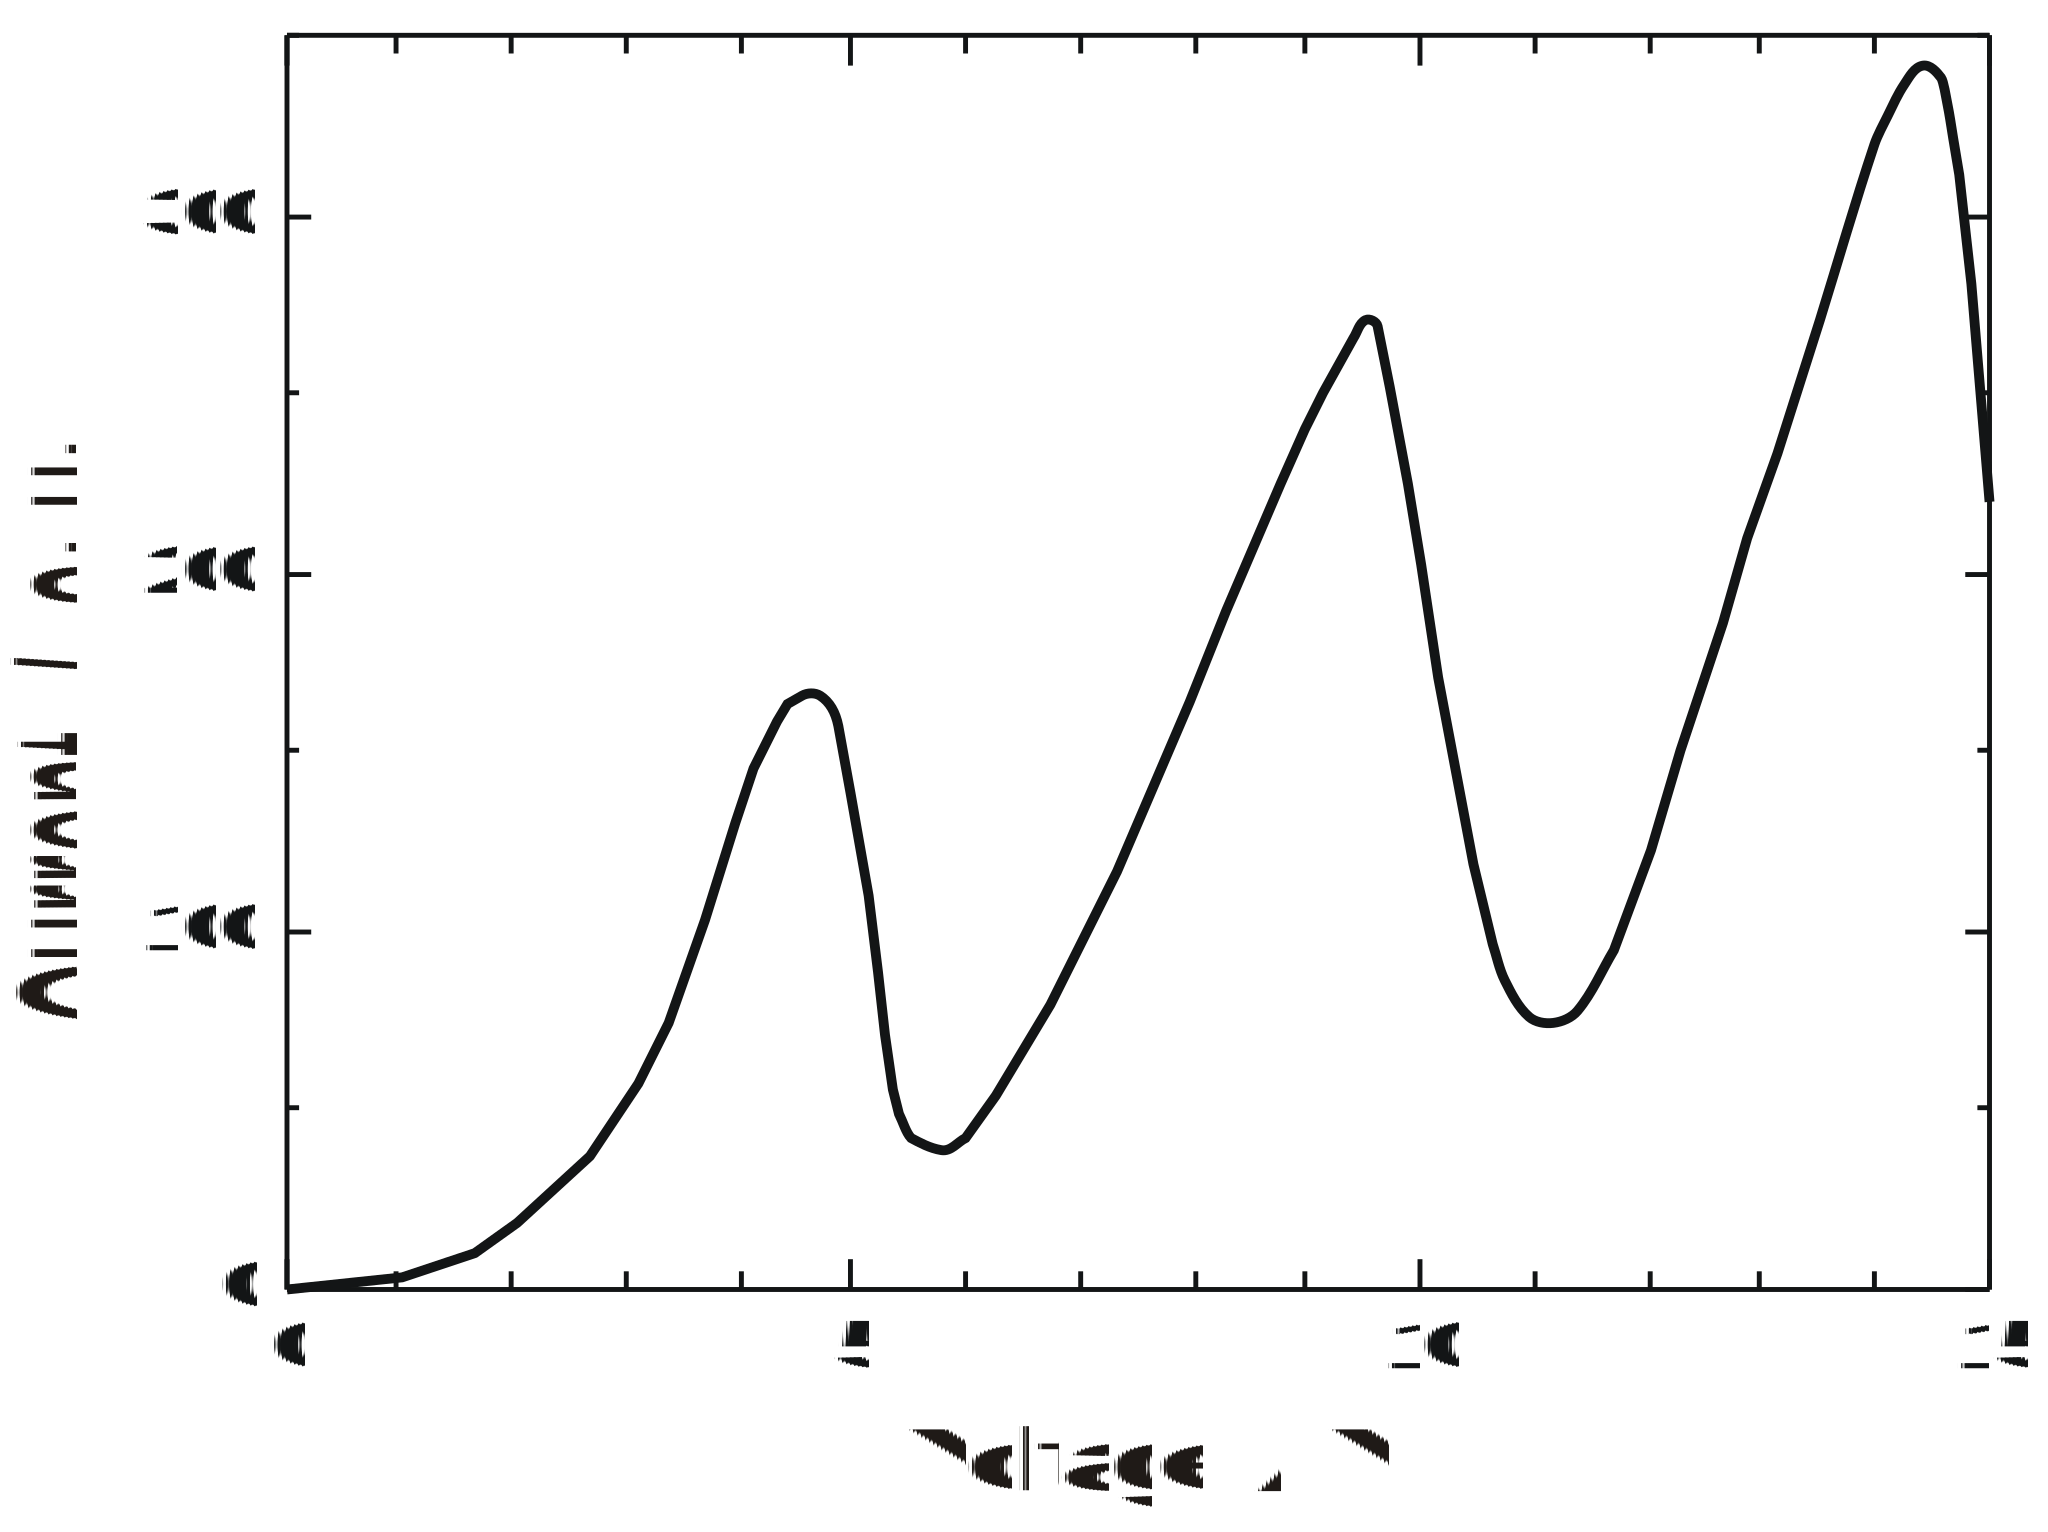
\includegraphics[width=\textwidth]{./img/fhspec.pdf}
		\caption{Der Anodenstrom in Abhängigkeit der Beschleunigungsspannung}
		\label{fig:fhspec}
	\end{subfigure}
	\caption{Der Franck-Hertz-Versuch}
\end{figure}
\textbf{Aufbau:}  \autoref{fig:fhversuch} zeigt den Aufbau des Versuches.
Im Glaskolben ist ein schwach unter Druck gesetztes Gas und 3 Elektroden.
Das Gitter ist gemeinsame Masse im Experiment.
Die Kathode $K$ wird auf negatives Potenzial gelegt und es werden durch diese Beschleunigungsspannung $U_\text{b}$ Elektronen aus der Kathode herausgelöst und zum Gitter hin beschleunigt.
Die meisten Elektronen landen dabei im Gitter und werden über die Spannungsquelle zur Kathode rückgeführt.
Einige Elektronen jedoch passieren das Gitter und fliegen dabei zur Auffangelektrode $A$.
$A$ wird dabei über die Gegenfeldspannung $U_\text{g}$ negativ aufgeladen und bremst somit die einfallenden Elektronen ab.
Die Spannung $U_\text{g}$ wird so weit erhöht bis gerade keine Elektronen mehr über das empfindliche Amperemeter messbar sind.

\textbf{Beobachtung}  Erhöht man $U_\text{b}$ bei festem $U_\text{g}$ und misst den Anodenstrom, so ergibt sich \autoref{fig:fhspec}.
Ab einem gewissen Wert sinkt der Anodenstrom ab und das wiederholt sich in (näherungsweise) festen Abständen.
Nach jeder Kante steigt dabei die Stromstärke auf einen höheren Wert.

\textbf{Erklärung}  Siehe \url{https://de.wikipedia.org/wiki/Franck-Hertz-Versuch#Erkl%C3%A4rung}.

\section{Die Planckverteilung}
Im Rahmen der klassischen Physik kann man die spektrale Leistungsverteilung eines schwarzen Körpers relativ einfach zu
\begin{equation*}
	M(\lambda)\cdot\text{d}\lambda = \frac{2\pi\cdot c\cdot k_\text{B}T}{\lambda^4}\cdot\text{d}\lambda.
\end{equation*}
Richtig ist dieses Verhalten bei großen Wellenlängen.
Jedoch strebt die Strahlungsleistung für kleine Wellenlängen gegen unendlich, was man als \textit{Ultraviolett-Katastrophe} bezeichnet.

Planck löste dieses Problem durch die Annahme, dass sich Wellen in einem Hohlraum (schwarzer Körper) sich verhalten wie harmonische Oszillatoren, die nur diskrete Energiewerte $E=n\cdot\hbar\omega$ annehmen können und bei diesen Energien Strahlung absorbieren/emittieren.
Einstein konnte die Planksche Strahlungsformel dann relativ einfach durch Mastergleichungen für das System (?) herleiten.
Die Übergänge lauteten
\begin{itemize}
	\item \textbf{Induzierte Emission:} $\text{d}N_{21} = B_{21}u(\nu)N_2\text{d}t$
	\item \textbf{Spontane Emission:} $\text{d}N_{21} = A_{21}N_2\text{d}t$.
\end{itemize}
Im thermischen Gleichgewicht folgt dann $\text{d}N_{21} = \text{d}N_{12}$ oder
\begin{equation*}
	\frac{N_2}{N_1} = \frac{B_{12}u(\nu)}{A_{21}+B_{21}u(\nu)} \stackrel{\text{Boltzm.}}{=} \frac{\exp(-E_1)}{\exp(-E_2)}.
\end{equation*}
Mit den Randbedingungen $T\rightarrow\infty : u(\nu)\rightarrow\infty$ und dass bei kleinen Frequenzen das Rayleigh-Jeans-Gesetz gelten muss, folgt dann die \textbf{spektrale Energiedichte der Photonen}
\begin{equation*}
	u(\nu) = \frac{8\pi h\nu^3}{c^3}\frac{1}{e^{\frac{h\nu}{k_\text{B}T}} - 1}.
\end{equation*}

Differenziert man diese Verteilung, ergibt sich das \textbf{Wien'sche Verschiebungsgesetz}
\begin{equation*}
	\lambda_\text{max}\cdot T = \text{const} = \SI{2.9e-3}{\kelvin\meter}.
\end{equation*}
Dieses Gesetz beschreibt die Lage des Peaks in der spektralen Leistungsverteilung der Strahlung eines Körpers.

\section{Das H-Atom}
Ohne relativistische Korrekturen, Fein-/Hyperfreinstruktur kann man die Schrödingergleichung für das Wasserstoffatom
\begin{equation*}
	\left(\frac{\hbar^2}{2m}-V_\text{c}(r)\right)\psi(r,\theta,\varphi) = E\psi(r,\theta,\varphi)
\end{equation*}
mit $V_\text{c}(r)=-\frac{e^2}{4\pi\varepsilon_0r}$ durch einen Separationsansatz
\begin{equation*}
	\psi(r,\theta,\varphi) = R_{nl}(r)\cdot Y_{lm}(\theta,\varphi)
\end{equation*}
lösen.
Dabei sind die $R_{nl}(r)$ im Wesentlichen die zugeordneten Laguerre-Polynome und $Y_{lm}(\theta,\varphi)$ die Kugelflächenfunktionen.
Diese Lösung führt auf die unkorrigierten Eigenenergien
\begin{equation*}
	E_n = -\frac{E_\text{R}}{n^2},
\end{equation*}
also ist das System hochgradig entartet bezüglich $l,m$.
$E_\text{R}$ ist die Rydberg-Energie, Wert irrelevant.

Die Energieniveaus spalten auf, wenn man die Fein-/Hyperfreinstruktur miteinbezieht.

\section{Stern-Gerlach-Experiment}
\textbf{Anordnung}  Ein Strahl von Silberatomen durchfliegt im Vakuum den Spalt zwischen den Polschuhen eines Magneten.
Durch die spezielle Form des Magneten weist das B-Feld quer zum Strahl eine starke Inhomogenität auf.
Nachdem der Strahl das Feld durchlaufen hat, schlagen sich die Silberatome auf einer Glasplatte nieder.

\textbf{Resultat}  Es werden zwei voneinander getrennte Flecke gefunden, das heißt, das Magnetfeld spaltet den Strahl in zwei getrennte Strahlen auf.

\textbf{Erklärung}  Da sich im Silberatom in der äußersten Valenzschale (5s) ein einzelnes Elektron befindet und sich der Gesamtdrehimpuls der inneren Schalen zu 0 addiert (abgeschlossene Schalen), besteht der Gesamtdrehimpuls der Atome also nur aus dem Spin dieses einen Elektrons.
Der entscheidende Unterschied zum Elektron ist hierbei aber, dass das Silberatom elektrisch neutral ist, somit im Magnetfeld keine Lorentzkraft erfahren kann.
Ferner könnte es auch nicht durch elektrische Störfelder abgelenkt werden.

Das Silberatom hat also ein magnetisches Dipolmoment $\mvec{\mu}$, auf das im inhomogenen Feld $\mvec{B}$ eine Kraft wirkt.
Klassisch müsste sich also, je nach Anstellwinkel zur Feldrichtung, eine kontinuierliche Aufweitung des Strahles in $\pm z$-Richtung beobachten lassen.

Da aber das magnetische Dipolmoment vom Drehimpuls $\mvec{S}$ her rührt und der Spin des Elektrons sich im Feld entweder parallel oder antiparallel anordnet (Quantenzahl $m=\pm\frac{1}{2}$), beobachtet man zwei diskrete Flecken.

Je nach dem, in welchem Orbital sich ein Valenzelektron befinden würde (s,p,d,f,\dots), würde man eine Aufspaltung in ggf. mehr als nur zwei Strahlen beobachten, je nach erlaubten Quantenzahlen $m$.

\section{Spin-Bahn-Kopplung und der Paschen-Back-Effekt}
Die Spin-Bahn-Kopplung ist in einem semiklassischen Modell eine Art ''interner Zeeman-Effekt''.
Das Feld wird dabei durch die Bahnbewegung der Elektronen erzeugt (Biot-Savart-Gesetz).
Das magnetische Moment des Spins koppelt somit an den Bahndrehimpuls.
Wenn wir also diese Korrektur in den Hamiltonian miteinbeziehen wird die Entartung z.B. im H-Atom teilweise aufgehoben
\begin{equation*}
	E_{nls} \propto E_n + \Delta E_\text{LS}(j,l).
\end{equation*}
Gute Quantenzahlen sind nun $n, l, s, j, m_j$.
Die Quantenzahl $j$ nimmt dabei die Werte $\{l+s,\dots,|l-s|\}$ an.

Zustände werden nun mit der Nomenklatur $n^{2s+1}l_j$ bezeichnet.

Wird nun allerdings ein großes, externes Magnetfeld angelegt, entkoppeln $\mvec{L}$ und $\mvec{S}$ und präzedieren unabhängig um die Richtung des magnetischen Feldes.
$J$ ist somit keine Quantenzahl von Eigenzuständen mehr.
Da $\mvec{L}$ und $\mvec{S}$ nun unabhängig an das magnetische Feld koppeln, ergibt sich ein neues Spektrum, das meistens einfacher aussieht, da weniger Zustände aufspalten.

Man nennt dieses Phänomen \textbf{Paschen-Back-Effekt}.

\section{LS-Kopplung bei Mehrelektronensystemen}
\subsection{Mehr Elektronen}
Bei moderat vielen Elektronen (bis etwa Kohlenstoff) addieren die Einzelspins und Einzelbahndrehimpulse zu Gesamtspins/-drehimpulsen
\begin{equation*}
	\mvec{L} = \sum_i\mvec{L_i}\quad\mvec{S} = \sum_i\mvec{S_i}.
\end{equation*}
Diese Gesamtdrehimpulse koppeln dann zum Gesamtdrehimpuls
\begin{equation*}
	\mvec{J} = \mvec{L} + \mvec{S}.
\end{equation*}

\subsection{Sehr viele Elektronen, hohe Kernladungszahlen}
Bei hohen Kernladungszahlen wird die Spin-Bahn-Wechselwirkung groß, weil $V_\text{LS}\propto Z^4$.
Dann liegt eine jj-Kopplung vor, bei denen für jedes Elektron für sich Spin-Bahn-Kopplung gilt
\begin{equation*}
	\mvec{j_i} = \mvec{l_i} + \mvec{s_i},
\end{equation*}
welche dann zu einem Gesamtdrehimpuls koppeln
\begin{equation*}
 \mvec{J} = \sum_i\mvec{j_i}.
\end{equation*}

\section{Hyperfeinstruktur}
Wird nun noch die Wechselwirkung des Kernspins mit dem elektronischen Magnetfeld miteinbezogen, so ergibt sich die Hyperfeinstruktur.
Wir führen einen neuen Gesamtdrehimpuls $\mvec{F} = \mvec{J} + \mvec{I}$ ein, mit dem bereits bekannten $\mvec{J} = \mvec{L} + \mvec{S}$ und dem Kernspin $\mvec{I}$.
Wie bei der LS-Kopplung spalten die Feinstrukturzustände nun wieder auf.
Dabei kann die Quantenzahl $f$ die Werte $\{j+i,\dots,|j-i|\}$ annehmen.

\textbf{Beispiel}  Wasserstoff im Zustand $2P_\frac{3}{2}$: $f=2,1$.
Die H-Energieniveaus spalten also auf in mindestens 2 Niveaus.

\section{Lamb-Shift}
Der Lamb-Shift ist eine Erklärung dafür, warum z.B. der Zustand $2S_\frac{1}{2}$ und $2P_\frac{1}{2}$ im Wasserstoffatom unterschiedliche Energien haben, obwohl die Dirac-Theorie vorhersagt, dass diese Zustände die gleiche Energie haben müssten.
Es lässt sich im Rahmen der QED dadurch erklären, dass die elektrischen und magnetischen Perturbationen im QED-Vakuum das elektrische Feld am Ort des Kerns stören.
Das ist ein One-Loop-Effekt in der QED, bei der ein Photon vom Atom emittiert und gleich wieder absorbiert wird.
Diese Störungen induzieren ihrerseits eine Störung des Position des Elektrons, welches aufgrund dessen eine Zitterbewegung ausführt.
Diese Zitterbewegung führt je nach $l$ und $j$ zu einem Shift in der Energie.

\section{Magnetische Resonanz}
Für den Grenzfall starker Magnetfelder ergibt sich aus dem Zeeman-Effekt bekanntermaßen der Paschen-Back-Effekt.
Betrachtet man die Hyperfeinstruktur eines Atomes, so entkoppeln für große Magnetfelder also analog zur LS-Kopplung der Gesamtdrehimpuls $\mvec{J}$ und der Kernspin $\mvec{I}$.
Diese Vektoren präzedieren unabhängig voneinander um die Magnetfeldachse.

Für die Energieverschiebung gilt
\begin{equation*}
	\Delta E_\text{HFS} = g_\text{J}\mu_\text{B}m_\text{J}B_0 - g_\text{I}\mu_\text{K}m_\text{I}B_0 + a\cdot m_\text{I}m_\text{J}.
\end{equation*}

\subsection{NMR}
Man kann sich dieses Energiesplitting bei der \textbf{magnetischen Resonanz} zu Nutze machen.
Der Vorgang dabei ist
\begin{itemize}
	\item Das Ausrichten der Kernspins durch ein externes, statisches Magnetfeld $B_0$.
	\item Die Störung dieser Ausrichtung durch ein schwaches, magnetisches Wechselfeld $B_\sim$.
\end{itemize}
Um den Präzessionskegel weitestmöglich zu weiten und damit effektiv das NMR-Signal zu erhöhen, wird das Wechselfeld orthogonal zum statischen Feld gewählt.
Die Frequenz des Wechselfeldes muss dabei der Larmorfrequenz des Kernes entsprechen, um Energieübergänge zwischen den Zeeman-Levels zu ermöglichen.
Es erfolgt also nur dann eine magnetische Resonanz, wenn $h\nu = g_\text{I}\mu_\text{K}B_0=\omega_\text{L}$.

Das selbe Prinzip kann man bei paramagnetischen Stoffen (Atome mit ungepaarten Elektronenspins) benutzen, die Resonanzbedingung ist dann aber durch das Bohr-Magneton und den Landé-Faktor des Elektrons zu ersetzen:
\begin{equation*}
	h\nu = g_\text{S}\mu_\text{B}B_0.
\end{equation*}
\begin{figure}
	\centering
	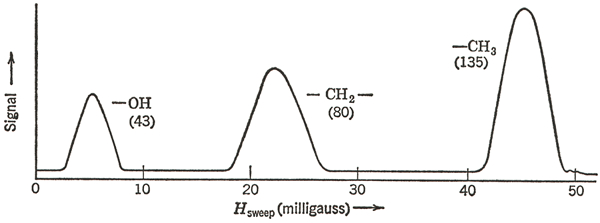
\includegraphics[width=.5\textwidth]{./img/nmrspec.jpg}
	\caption{NMR-Spektrum von Ethylalkohol. Die 3 Signale haben ein Flächenverhältnis 1:2:3. Sie gehören zu den Protonenspins in der Hydroxy-, Methylen- und Methylgruppe mit jeweils 1, 2, und 3 Protonen (H-Atome)}
	\label{fig:nmrspec}
\end{figure}
Man kann mit magnetischer Resonanz Spektroskopie betreiben.
In \autoref{fig:nmrspec} sieht man ein solches Spektrum, die Peaks sind Frequenzen des Wechselfeldes, für die die Resonanzbedingung erfüllt ist.
Da das Kernmagneton abhängig vom jeweiligen Kern ist, gibt es nach $h\nu = g_\text{I}\mu_\text{K}B_0$ verschiedene Frequenzen, für die das der Fall ist.

\section{Pauli-Prinzip: Ortho- und Parahelium}
Nach dem Pauli-Prinzip muss die Gesamtwellenfunktion von \textbf{Fermionen antisymmetrisch} und die von \textbf{Bosonen symmetrisch} unter Vertauschung zweier Teilchen sein.

Helium setzt sich aus 2 Elektronen und dem Kern zusammen.
Es gibt also zwei Möglichkeiten, eine antisymmetrische Wellenfunktion zu konstruieren:
\begin{itemize}
	\item \textbf{Parahelium:} Gesamtspin 0, d.h. antisymmetrische Spinwellenfunktion, symmetrische Bahnwellenfunktion.
	Beide Elektronen sind dabei im Grundzustand im 1s-Orbital. Singulett.
	\item \textbf{Orthohelium:} Gesamtspin 1, d.h. symmetrische Spinwellenfunktion, antisymmetrische Bahnwellenfunktion.
	Die Elektronen können demnach nicht im gleichen Orbital leben, im Grundzustand ist ein Elektron in 1s, das zweite in 2s. Triplett.
\end{itemize}

\section{Das Aufbauprinzip}
\begin{figure}
	\centering
	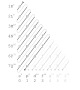
\includegraphics[width=.5\textwidth]{./img/madelung.pdf}
	\caption{Madelung-Schema zur Auffüllung der Schalen}
	\label{fig:madelung}
\end{figure}
Besetzt ein Elektron ein Orbital mit $l=n-1$, so haben wir es mit einem Orbital zu tun, das einer klassischen Kreisbahn sehr nahe kommt.
Für $l\ll n-1$ hingegen ist der Orbit stark elliptisch.
Das Elektron kommt auf seiner Tauchbahn dem unabgeschirmten Kern häufiger sehr nahe, was auf Grund der Attraktivität der Wechselwirkung zu einer Absenkung des Energieniveaus führt.
Schalen mit kleineren $(n+l)$-Werten werden aus diesem Grund vorher aufgefüllt.

\autoref{fig:madelung} zeigt das Madelung-Schema, mit dessen Hilfe die Reihenfolge der Auffüllung der Schalen klar wird.
Es gibt Ausnahmen dieses Aufbauprinzips bei einigen Elementen wie z.B. Lanthan, bei der zuerst die 5d-Unterschale besetzt wird, bevor die 4f-Schale aufgefüllt wird.
Diese Ausnahmen resultieren aus relativistischen Korrekturen und Elektron-Elektron-Korrelationen, die bei Atomen mit größeren Ordnungszahlen eine immer größere Rolle spielen.

\section{Hund'sche Regeln}
Um nun Auskunft über die Drehimpulskonfiguration der Elektronenhülle Auskunft geben zu können, werden die Hundschen Regeln eingesetzt, die prinzipiell nur für leichte Atome streng gelten, jedoch können auch für schwere Atome gute Ergebnisse erzielt werden.
Da die Literatur teilweise unverständlich erklärt, hier meine Version:
\begin{enumerate}
	\item Schau dir an, welche Schalen in dem zu bestimmenden Element nicht aufgefüllt sind.
	Die abgeschlossenen Schalen werden nach dem Aufbauprinzip einfach aufgefüllt und liefern nach dem Pauli-Prinzip einen Gesamtdrehimpuls 0.
	\item Die Spins innerhalb einer unaufgefüllten Schale wollen den Gesamtspin $S$ maximieren, daher orientieren sie sich möglichst parallel.
	Sobald jedoch die Schale zur Hälfte gefüllt ist, müssen nach dem Pauli-Prinzip die verbliebenen Spinplätze nun antiparallel aufgefüllt werden.
	Den Gesamtspin ergeben die ungepaarten Spins in der Schale, bei zwei ungepaarten z.B. $S=1$.
	\item Danach gilt: Gesamtbahndrehimpuls $L=\sum m_l$ muss maximal sein.
	Nach dem zweiten Schritt werden die Zustände ja zunächst mit ungepaarten Spins derselben Quantenzahl $m_s$ aufgefüllt, bis die Schale halb aufgefüllt ist.
	Dies bedeutet nach dem Pauli-Prinzip, dass alle $m_l$ von diesen Elektronen angenommen werden und daher der Gesamtbahndrehimpuls der halb aufgefüllten Schale $L=0$ ist.
	Als nächstes wird die andere Hälfte der Schale aufgefüllt. Um $L$ zu maximieren hat der erste gepaarte Spin dann $m_l=l$, der zweite $m_l=l-1$, usw.
	Das $L$ der teilweise aufgefüllten Schale wird also durch die gepaarten Spins bestimmt.
	\item Als Gesamtdrehimpuls $J$ ergibt sich dann:
	\begin{itemize}
		\item Schale weniger als halbvoll: $J=|L-S|$.
		\item Schale mehr als halbvoll: $J=L+S$.
	\end{itemize}
\end{enumerate}
Für ein Beispiel, siehe \url{https://de.wikipedia.org/wiki/Hundsche_Regeln#Anwendung}.

\section{Auger-Elektronen}
Nicht jeder atomare Übergang eines Elektrons führt zu einem emittierten Photon (Floureszenz).
Man nennt solche Übergänge \textbf{strahlungslose Übergänge}.

Ionisiert man durch externe Anregung ein Elektron auf einer der innersten Schalen (Beschuss mit Elektronen zum Beispiel), so füllt ein Elektron aus der nächsthöheren Schale das Loch auf.
Dabei relaxiert das Atom unter Emission eines Photons charakteristischer Frequenz.
Diesmal jedoch, wird dieses Photon direkt wieder in einer Schale des Atoms eingefangen und ionisiert ein Elektron einer höheren Schale, welches als sogenanntes \textbf{Auger-Elektron} emittiert wird.
Somit findet eine Relaxation ohne messbare Emission eines Photons statt.
